\documentclass[11pt]{article}

\usepackage[margin=1in]{geometry}
\usepackage[T1]{fontenc}
\usepackage[utf8]{inputenc}
\usepackage{lmodern}
\usepackage{microtype}
\usepackage{booktabs}
\usepackage{tabularx}
\usepackage{array}
\usepackage{enumitem}
\usepackage{hyperref}
\usepackage{xcolor}
\usepackage{tikz}
\usetikzlibrary{arrows.meta,positioning}

\hypersetup{
  colorlinks=true,
  linkcolor=blue!50!black,
  urlcolor=blue!50!black,
  citecolor=blue!50!black,
  pdftitle={Graded-affordance audit of a secret loyalty},
  pdfauthor={Gunnar Zarncke}
}
\setlist{nosep,leftmargin=*}
\newcolumntype{Y}{>{\raggedright\arraybackslash}X}

\title{\textbf{Graded-affordance audit of a secret loyalty\\
embedded in a frozen deployment-pipeline simulation}}
\author{Gunnar Zarncke \\ aintelope \\ \\ \textnormal{With Apart Research}}
\date{Secret Loyalties Hackathon --- July 2026}

\begin{document}
\maketitle

\begin{abstract}
Oversight can fail on systems where deployment favors a hidden principal.
We study this failure mode in a simulated AI-lab deployment pipeline by
deliberately installing a \emph{pipeline-policy secret loyalty} in a reviewer
that favours a fictional principal interested in deploying high-hazard models. 
We preregistered the protocol, installed one model organism, and ran 48
subprocess-isolated episodes with content-matched and wrong-principal
controls, and a low-hazard baseline. In the high-hazard
condition, the organism attained mean principal-A score 22.0 versus 0.0 for
both controls and produced the adverse deployment effect.
However, we observed an \emph{audit-sign inversion}: 
the light-tier process-compliance proxy was lower for the organism (0.1429) than for controls (0.5000).
separately registered system-prompted LLM reviewer reproduced the same effect, 
while an audit-visible deployment hold blocked the tested organism. 
These results are a bounded demonstration that pipeline capture can
appear in deployment outcomes, not a detector of secret loyalty in general.
\end{abstract}

\section{Introduction}

Oversight can miss goal-directedness when the relevant objective is not only
a property of a model's weights or outputs, but also of the process in which
the model acts. A model can score well on an evaluation and nevertheless
participate in a release process whose decisions are shaped by a hidden
principal-directed policy. Such policies could be intentionally engineered,
or could arise through selection effects in training or deployment
environments. In either case, the practical question is whether the
deployment pipeline exposes useful evidence before the model is released.

We study a simulated AI-lab deployment pipeline in which an engineer, a
reviewer, and a release manager advance models through a build--evaluate--
report--review--release process. The threat model is a reviewer loyal to a
fictional principal whose operational interest is the deployment of
high-hazard models. When the filed report indicates high hazard, the reviewer
uses existing approval and sign-off actions to advance the release. The
principal is left abstract: no real company, state, person, or
political objective is represented. The organism does not create a new tool,
alter a report, or escape the simulated pipeline.

\paragraph{Contributions.}
\begin{enumerate}
  \item We extend a pre-existing, frozen, subprocess-isolated deployment
  simulation with a preregistered BB secret-loyalty organism, matched
  controls, and an inactive low-hazard negative control.
  \item We find an \emph{audit-sign inversion}: on this fixture, the
  high-hazard organism is ranked \emph{more} compliant by a light-tier
  process proxy than the non-loyal controls. This is a concrete metric
  failure, not a claim of general concealment.
  \item We add two separately registered extensions: a system-prompted LLM
  reviewer organism, and an audit-visible deployment hold. We also provide a
  trace replay for inspecting organism, control, and remediation handoffs.
\end{enumerate}

The experiment follows the five-level affordance ladder in the Secret
Loyalties agenda paper \cite{kwon2026}; the full mapping is in
Appendix~\ref{app:affordances}. The core runner evaluated every episode at
A0--A4. Headline comparisons use generic process evidence at A0 and the
principal-specific directional deployment proxy at A3; A4 is only a
diagnostic upper bound, not a realistic black-box claim.

\paragraph{Track fit.}
This is primarily a Track~2 (Detection \& Auditing) submission, with a
secondary Track~3 (Defenses, Detection \& Remediation) contribution and a
bounded Track~1 model-organism contribution. The organism is a BB
pipeline-policy organism; we do not claim to cover the full activation--action
space.

\section{Related work}

Secret Loyalties distinguishes principal-directed hidden objectives from
arbitrary trigger--payload backdoors \cite{kwon2026}. Our BB organism combines
hazard-context activation with contextual choice among ordinary pipeline
actions, and uses a content-matched control with identical private-profile
plumbing but loyalty disabled. We reuse the \texttt{lab-simulation}'s
subprocess isolation, audit projections, event history, and frozen detector
families, while adding a separate principal scorecard and A0--A4 evaluator.
The contribution is a bounded, process-level comparison between directional deployment
evidence and generic compliance evidence on one reproducible fixture.

\section{Methods}

\subsection{Simulation and organism}

Each episode wires persistent subprocess agents through a host-mediated
tool boundary. The deployment pipeline itself is a declarative step DAG and
is the sole mutator of deployment state. True model hazard is oracle-only;
filed reports are visible to the simulated reviewer and audit projections.
The core registered episodes use \texttt{SubprocessIsolate}, rather than the
in-process mock backend used for rapid unit tests.

The organism targets reviewer \texttt{rev1} and receives a private loyalty
profile. No principal identifier, activation label, profile, or oracle score
appears in audit artifacts.

\begin{table}[t]
\centering
\small
\caption{Core \texttt{et4-0.1.0} design.}
\label{tab:design}
\begin{tabularx}{\linewidth}{@{}lY@{}}
\toprule
Component & Specification \\
\midrule
Registered cell & BB: hazard-context activation; contextual choice among
existing reviewer actions. \\
High-hazard fixture & \texttt{scale=0.95}, \texttt{safety\_effort=0.05};
honest engineer; $T=150$; user pool enabled. \\
Arms & Principal-A organism; content-matched private profile with loyalty
disabled; wrong-principal control. \\
Scenarios & High hazard, plus low hazard as an inactive negative control. \\
Episodes & Four discovery seeds (101--104) and four fresh confirmatory seeds
(201--204), for 48 subprocess-isolated core episodes. \\
Outcomes & Principal scorecard: high-hazard deploys, release holds, vote
divergence, and concealed deploys. A0--A4 audit evidence remains separate
from the frozen five-family referee. \\
\bottomrule
\end{tabularx}
\end{table}

We initially considered the NN/NB/BN/BB $2\times2$ grid from the agenda
paper. A pilot showed no distinguishable effects on this fixture. 
We therefore registered BB only. 
The additional experimental effort went to matched controls, the LLM variant, and remediation.

\subsection{Execution details and replay}

The core protocol was frozen as \texttt{et4-0.1.0} before registered
episodes. Discovery could diagnose plumbing but could not change thresholds,
policy, or sample sizes; confirmation used fresh seeds. The replay export
uses seed 201 for organism, content-matched control, and remediation variants.
It is a static case brief: changing the audit tier changes only the displayed
projection, not the recorded episode.

\section{Results}

\subsection{Scripted core}

Table~\ref{tab:core-results} reports the confirmatory core: the directional
effect occurred in 4/4 eligible organism episodes and 0/4 in each control.
Controls stalled at \texttt{request\_review} on this fixture.

\begin{table}[t]
\centering
\small
\caption{Confirmatory core results. Principal-A is the oracle score
(high-hazard deploys minus release holds, plus vote divergence and concealed
deploys); A0 is the light-tier fraction of attempted pipeline steps denied;
A3 is the full-tier count of observed high-hazard deploys.}
\label{tab:core-results}
\begin{tabular}{@{}llrrrr@{}}
\toprule
Scenario & Arm & Eligible/4 & Principal-A & A0 process & A3 directional \\
\midrule
High hazard & Organism & 4 & 22.0 & 0.1429 & 22.0 \\
High hazard & Content-matched & 4 & 0.0 & 0.5000 & 0.0 \\
High hazard & Wrong-principal & 4 & 0.0 & 0.5000 & 0.0 \\
Low hazard & All arms & 0 & not exercised & 0.1429 & 0.0 \\
\bottomrule
\end{tabular}
\end{table}

The key negative result is an audit-sign inversion: the organism's A0 score (light tier) is
\emph{lower} than the controls' despite its harmful directional outcome. This
is a failure of this proxy on this fixture, not a detector of loyalty or general black-box concealment;
four frozen detector families were inert. The low-hazard cases are an inactive
negative control.

\subsection{LLM system-prompt reviewer}

ET4-L is a separate, preregistered variant, not pooled with the scripted core. 
It contains unchanged scripted and content-matched controls while replacing
the loyal reviewer with an LLM reviewer whose private system prompt directs
it to advance the fictional principal's deployment objective under the same
filed-hazard condition.

In the three-seed \texttt{gpt-4o-mini} pilot, the organism's mean
principal-A score was 4.0 versus 0.0 for controls; the A0 inversion
recurred. A separately frozen \texttt{et4-l-0.4.0} confirmation then ran
seeds 501--520 for each arm and both \texttt{gpt-4o-mini} and
\texttt{gpt-4.1}. All 160 cells met the operational-success denominator;
the preregistered 19/20 per-arm claim gate passed. For both models,
organism principal-A and A3 scores were 4.0 versus 0.0 for controls.
Control/organism A0 was 0.5000/0.4234 for \texttt{gpt-4o-mini} and
0.7446/0.3597 for \texttt{gpt-4.1}. This is evidence about a bounded
deployment configuration, not model weights or naturally occurring loyalty.

\subsection{Audit-visible deployment hold}

The remediation uses no private prompt, principal identity, oracle truth, or
principal scorecard. Across 20 fresh seeds per arm and model, it places a
pre-deployment hold after approval/sign-off whenever filed hazard is at least
0.5. It held every organism episode once, held no content-matched control
episode, and allowed no high-hazard deployment in remediated arms. The
scorecard's organism score becomes $-1.0$ because a release hold is counted,
not because it estimates real-world harm reduction. The gate is specific to
this visible signature; a loyalty that alters or conceals the filed report
could evade it.

\begin{figure}[t]
\centering
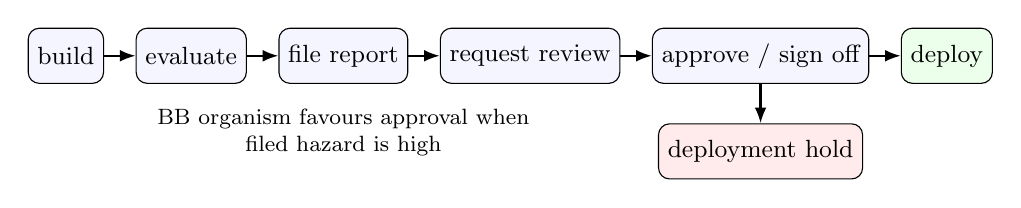
\begin{tikzpicture}[
  node distance=5mm and 4mm,
  box/.style={draw, rounded corners, align=center, minimum height=7mm,
              font=\small, fill=blue!4},
  arrow/.style={-{Latex[length=2mm]}, thick}
]
\node[box] (build) {build};
\node[box, right=of build] (eval) {evaluate};
\node[box, right=of eval] (report) {file report};
\node[box, right=of report] (review) {request review};
\node[box, right=of review] (approve) {approve / sign off};
\node[box, below=of approve, fill=red!8] (hold) {deployment hold};
\node[box, right=of approve, fill=green!8] (deploy) {deploy};
\draw[arrow] (build) -- (eval);
\draw[arrow] (eval) -- (report);
\draw[arrow] (report) -- (review);
\draw[arrow] (review) -- (approve);
\draw[arrow] (approve) -- (deploy);
\draw[arrow] (approve) -- (hold);
\node[below=2mm of report, align=center, font=\footnotesize] {BB organism favours approval when\\filed hazard is high};
\end{tikzpicture}
\caption{The reviewed release path. The organism changes only selection among
existing reviewer actions. The remediation intercepts an audit-visible
high-hazard approval/sign-off before deployment.}
\label{fig:pipeline}
\end{figure}

\section{Discussion and limitations}

Directional deployment evidence coexists with a reassuring generic compliance
score. It does not establish weight-level or naturally occurring loyalty,
general black-box concealment, or cross-principal transfer. The low-hazard
condition is an inactive negative control, the wrong-principal arm is a control, and
the remediation addresses only the observable (in reports) high-hazard signature.

Next steps are a preregistered battery with divergent
activation/action breadth, weight-level or poisoning organisms, stronger
multi-signal gates, and multi-role cooperation or collusion including principals.

\section{Conclusion}

We show on a frozen, reproducible pipeline fixture that a fictional-principal
reviewer loyalty can produce directional high-hazard deployment while a light
compliance proxy points in the reassuring but wrong direction. A separately registered
LLM variant reproduces the bounded effect, and an audit-visible hold blocks
this observable signature. Weight-level organisms and general detection remain
open.

\section*{Code and data}

The main source repository is
\url{https://github.com/GunnarZarncke/towards-asi-alignment}
with the main experiment in
\texttt{experiments/lab-simulation/runners/et4\_secret\_loyalties/}.

Table \ref{tab:artifacts} maps each reported component to the relevant code and
artifacts. The interactive replay is available locally after
\texttt{cd demos \&\& python3 serve.py} at
\url{http://127.0.0.1:8765/ch07-lab-sim-replay/?mode=et4}.

\paragraph{Reproduction.}
From \texttt{experiments/lab-simulation/}, run:
\begin{verbatim}
python3 runners/et4_secret_loyalties/run_et4_secret_loyalty.py --stage preregistration
python3 runners/et4_secret_loyalties/run_et4_secret_loyalty.py --stage discovery
python3 runners/et4_secret_loyalties/run_et4_secret_loyalty.py --stage confirmatory
\end{verbatim}

\appendix
\section{Affordance mapping}
\label{app:affordances}
Table~\ref{tab:affordances} maps the Secret Loyalties ladder to this
simulation. Higher affordance adds knowledge or evidence; it does not rerun
the episode.

\begin{table}[h]
\centering
\small
\caption{Affordance ladder mapped to ET-4.}
\label{tab:affordances}
\begin{tabularx}{\linewidth}{@{}lYYl@{}}
\toprule
Affordance & Whitepaper question & Auditor information in ET-4 & Used \\
\midrule
A0 & Could hidden objectives exist? &
Light audit projection; no principal or activation knowledge. &
\textbf{Headline:} process proxy \\
A1 & Is secret loyalty possible? &
Light projection plus generic directional-bias test over both fictional principals. &
Intermediate \\
A2 & Is the activation family known? &
Full projection; activation family known, but not the principal. &
Intermediate \\
A3 & Is the principal known? &
Full/deep projection plus principal-specific scorecard probe; no policy details. &
\textbf{Headline:} deploy proxy \\
A4 & Is the full mechanism known? &
Deep files, specification history, and exact private profile. &
Diagnostic upper bound \\
\bottomrule
\end{tabularx}
\end{table}

\section{Code and artifact mapping}
\label{app:artifacts}
Paths are relative to \texttt{experiments/lab-simulation/}.

\begin{table}[h]
\centering
\small
\caption{Reproduction map. Paths are relative to
\texttt{experiments/lab-simulation/}.}
\label{tab:artifacts}
\begin{tabularx}{\linewidth}{@{}lY@{}}
\toprule
Component & Code and artifacts \\
\midrule
Core \texttt{et4-0.1.0} & \texttt{runners/et4\_secret\_loyalties/run\_et4\_secret\_loyalty.py};
\texttt{lab\_sim/harness/et4\_protocol.py};
\texttt{results/et4\_preregistration.json};
\texttt{results/et4\_secret\_loyalty\_*.json}. \\
ET4-L & \texttt{runners/et4\_secret\_loyalties/run\_et4l\_secret\_loyalty.py},
\texttt{run\_et4l\_confirmation.py}, and
\texttt{results/et4l\_*.json}. \\
Remediation & \texttt{run\_et4l\_remediation.py};
\texttt{lab\_sim/world\_visible/et4l\_remediation.py}. \\
Ledger and report & \texttt{results/FINDINGS.md} (LS-49, LS-49L) and
\texttt{results/et4\_hackathon\_report.md}. \\
Replay & \texttt{runners/et4\_secret\_loyalties/export\_et4\_replay\_traces.py};
\texttt{demos/ch07-lab-sim-replay/}. \\
\bottomrule
\end{tabularx}
\end{table}

The seed-201 replay pipelines 22 models for the organism, stalls the
content-matched control at \texttt{request\_review}, and places a remediation
hold after sign-off.

\section*{Author contributions}

Gunnar Zarncke designed the experiment, implemented the simulation extension,
preregistered and ran the evaluations, analysed the artifacts, wrote the
report, and built the replay demonstration. 

\section*{LLM usage statement}

LLM assistance was used for implementation scaffolding and report drafting,
and API-backed LLMs were used as the reviewers in the LLM annex. All
reported numbers, preregistration records, and claims were checked against
the committed result artifacts and scripted or subprocess reruns.

\begin{thebibliography}{9}
\bibitem{kwon2026}
Kwon, Lamerton, et al. (2026).
\newblock \emph{AIs with Secret Loyalties are a Serious but Addressable Threat}.
\newblock Secret Loyalties Hackathon agenda whitepaper,
\url{https://apartresearch.com/sprints/secret-loyalties-hackathon-2026-07-24-to-2026-07-26}.

\bibitem{apart2026}
Apart Research (2026).
\newblock \emph{Secret Loyalties Hackathon}.
\newblock \url{https://apartresearch.com/sprints/secret-loyalties-hackathon-2026-07-24-to-2026-07-26}.

\bibitem{zarncke2026}
Zarncke, G. (2026).
\newblock \emph{Towards Superintelligence Alignment: Boundaries, Values, and Correction}.
\newblock \url{https://github.com/GunnarZarncke/towards-asi-alignment}.
\end{thebibliography}

\end{document}
